\begin{frame}{Model Variables}
    Select indicator variables in addition to real GDP:
    \begin{itemize}
        \item rPCE (Real Personal Consumption Expenditures)
        \item rGCE (Real Government Consumption Expenditures)
        \item GPDI (Gross Private Domestic Investment)
    \end{itemize}
\end{frame}

\begin{frame}{Data Transformations}
    Real GDP and all of the variables have non-linear trends.
    
    To obtain stationary data for the VAR model, first take the log
    of each variable, and then the first difference:
    
    \begin{figure}[ht]
        \includegraphics<1>[width=8cm]{../img/rgdp.png}
        \includegraphics<2>[width=8cm]{../img/rgdp-log.png}
        \includegraphics<3>[width=8cm]{../img/rgdp-fdlog.png}
    \end{figure}
\end{frame}

\begin{frame}{ADF Test Results - Stationarity}
    Use the Augmented Dickey-Fuller test to verify that transformed
    variables are stationary:
    \begin{center}
    \begin{tabular}{cc}
        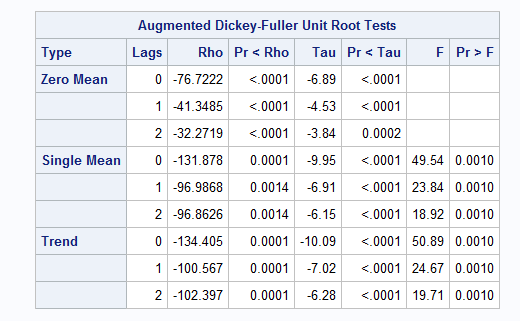
\includegraphics[width=0.30\textwidth]{../img/rgdp-fdlog-ADFtest.png} &
        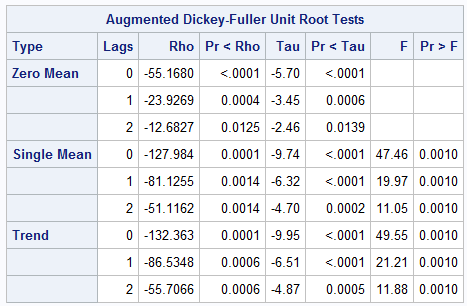
\includegraphics[width=0.30\textwidth]{../img/rpce-fdlog-ADFtest.png} \\
        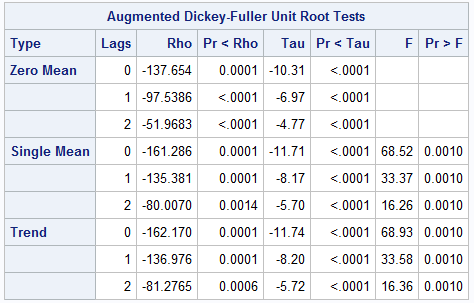
\includegraphics[width=0.30\textwidth]{../img/rgce-fdlog-ADFtest.png} &
        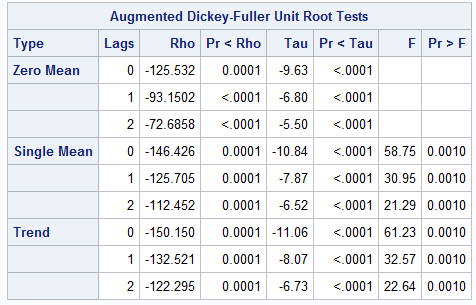
\includegraphics[width=0.30\textwidth]{../img/gpdi-fdlog-ADFtest.png} \\
        \multicolumn{2}{c}{\tiny \centering Clockwise from UL: rGDP, rPCE, GPDI, rGCE }
    \end{tabular}
    \end{center}
\end{frame}

\begin{frame}{AIC Test Results - P value}  
    Find the time-lag $p$ with the lowest Akaike Information Criterion:
    \begin{center}
    \begin{tabular}{|c|r|r|r|r|r|r|}
        \hline $p$ & 1 & 2 & 3 & \cellcolor{gray}\color{blue}4 & 5 & 6 \\
        \hline AIC & -44.9464 & -44.9059 & -44.9927 & \cellcolor{gray}\color{blue}-45.0499 & -44.9380 & -38.5330 \\
        \hline
    \end{tabular}
    \end{center}
    
    This suggests that a VAR(4) model is optimal.
\end{frame}


\begin{frame}{Model Solution} 
    Solve the VAR(4) model using Ordinary Least Squares (OLS):
    
    \begin{align*}
        log(rGDP)_t =  0.0002 
        + \left( -0.332, -0.191, -0.402, -1.314 \right) \cdot \vect{x}_{t-1} \\
        + \left(  0.005,  0.045, -0.135,  0.450 \right) \cdot \vect{x}_{t-2} \\
        + \left(  0.051, -0.430, -0.047,  0.570 \right) \cdot \vect{x}_{t-3} \\
        + \left(  0.195, -0.188,  0.225,  0.912 \right) \cdot \vect{x}_{t-4}
    \end{align*}
    
    \[ \text{with } \vect{x} = \begin{pmatrix} log(rGDP) \\ log(rPCE) \\ log(rGCE) \\ log(GPDI) \end{pmatrix} \]
\end{frame}
    
\begin{frame}{Statistical Significance}
    \begin{columns}[c]
    \column{0.7\textwidth}
        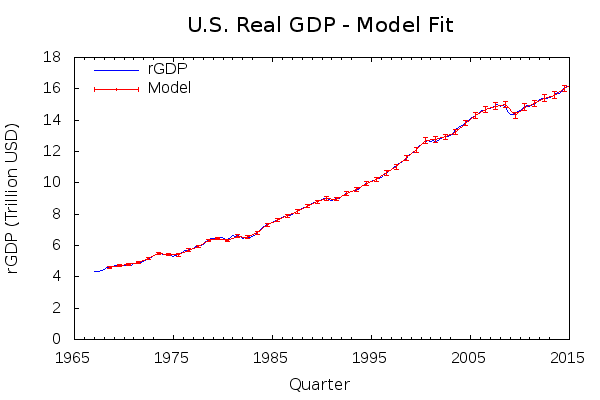
\includegraphics[width=\textwidth]{../img/model1-rgdp-fit.png}
    \column{0.3\textwidth}
        An excellent fit with historical rGDP values.
        
        \vspace{.9cm}
        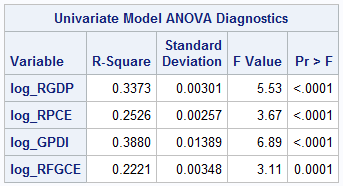
\includegraphics[width=\textwidth]{../img/model1-fitstats.png}
        
        \vspace{.9cm}
        RMS fit error: \[\sigma_\epsilon = 0.00301 \]
    \end{columns}
\end{frame}

\begin{frame}{Validating VAR Model Assumptions}
    Check the original assumptions about the residual error:
    \begin{align*}
        \expc{\epsilon_t} &= 0 \\
        \expc{\epsilon_t^2} &= \sigma_\epsilon^2 \\
        \expc{\epsilon_t \cdot \epsilon_{t-T}} &= 0 \text{ for } T \neq 0
    \end{align*}
    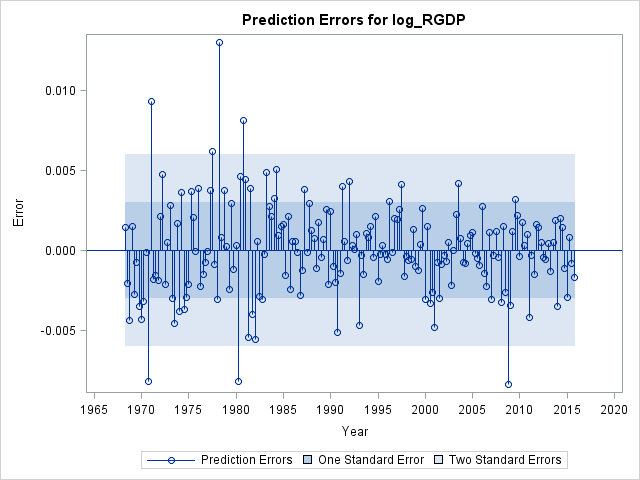
\includegraphics[width=0.6\textwidth,height=0.6\textheight]{../img/model1-residuals.png}
    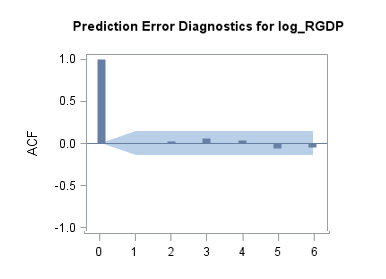
\includegraphics[width=0.4\textwidth]{../img/model1-residualdiagnostics.png}
\end{frame}

\begin{frame}{Analyzing Outliers}
    \begin{center}
        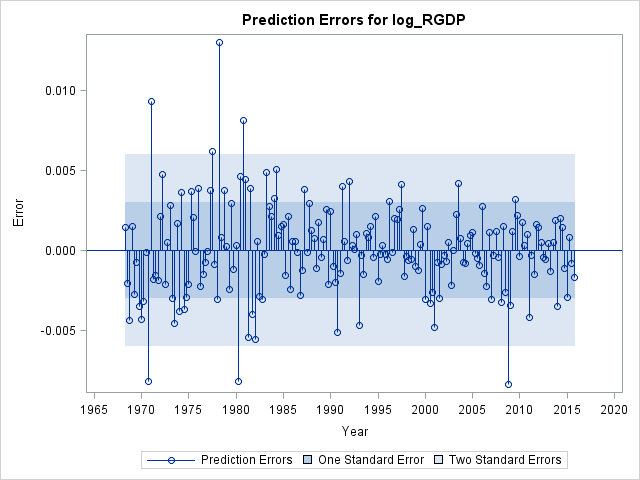
\includegraphics[width=0.6\textwidth,height=0.55\textheight]{../img/model1-residuals.png}
    \end{center}
    Notably, outliers occur mostly around recessionary periods:
    \begin{itemize}
        \item 1970-Q4, 1971-Q1: just after recessionary period (Dec 1969 - Nov 1970)
        \item 1980-Q2, 1980-Q4: during recessionary period (Jan - Jul 1980)
        \item 2008-Q4: during sub-prime mortgage crisis
    \end{itemize}
\end{frame}

\begin{frame}{Validating OLS Solution Assumptions}
    Check that residuals are normally distributed, as per OLS model:
    \begin{center}
        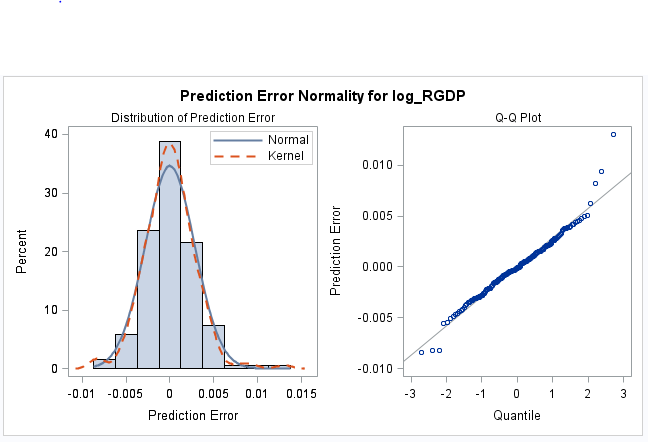
\includegraphics[width=0.7\textwidth]{../img/model1-errornormality.png}
    \end{center}
\end{frame}

\begin{frame}{Real GDP Forecast}

\begin{columns}[c]
    \column{0.7\textwidth}
        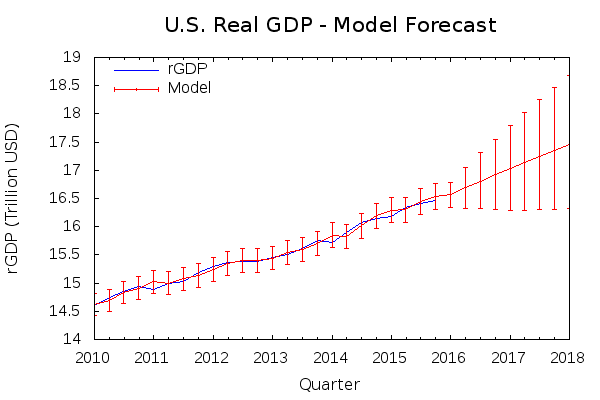
\includegraphics[width=\textwidth]{../img/model1-rgdp-forecast.png}
    \column{0.3\textwidth}
        \begin{table}
        \tiny
        \centering
        \begin{tabular}{c c c} 
            \bf{Quarter} & \bf{Forecast} & \bf{95\% Conf. Interval} \\ \hline
            2016-Q1 & 16.563 & 16.339 - 16.789 \\
            2016-Q2 & 16.687 & 16.330 - 17.051 \\
            2016-Q3 & 16.805 & 16.315 - 17.310 \\
            2016-Q4 & 16.919 & 16.309 - 17.552 \\
            2017-Q1 & 17.028 & 16.296 - 17.794 \\
            2017-Q2 & 17.136 & 16.293 - 18.023 \\
        \end{tabular}
        \end{table}
    \end{columns}
\end{frame}